\documentclass{newlayout}
%Bitte hier den enstprechenden Ort einsetzen z.B. Braunschweig und die Akademienummer
\Akademie{Rossleben}{2017}{5}

\usepackage[ngerman,english]{babel}
\usepackage{misc}
\usepackage{multicol}
\usepackage{booktabs}

\usepackage{color}% für Farben im allgemeinen
\usepackage{colortbl}

\usepackage{url}
\usepackage{breakurl}

\usepackage{units}

% hinzugef?gt, um Fehler 'pdfTeX error (font expansion): auto expansion is only possible with scalable' zu vermeiden
%\usepackage{lmodern}
\setkomafont{descriptionlabel}{\normalfont\bfseries}
\addtokomafont{paragraph}{\normalfont}
\usepackage{footnote}
\usepackage[flushmargin,hang,ragged]{footmisc}
\deffootnote{1em}{1em}{%
\textsuperscript{\thefootnotemark\ }
}

%\usepackage{amsmath}%wird automatisch durch newlayout.cls geladen
\usepackage{amsfonts}

%%%%%Mathe-Definitionen
\newtheorem{Def}{Definition}
\newtheorem{Sat}{Satz}
\newtheorem{Bew}{Beweis}

\setlength\abovedisplayshortskip{0pt}
\setlength\belowdisplayshortskip{0pt}
\setlength\abovedisplayskip{3pt}
\setlength\belowdisplayskip{3pt}
%%%%Ende Mathe-Definitionen

\begin{document}

 %   \input{titel}
 \setcounter{page}{3}

\setcounter{tocdepth}{1}
 \tableofcontents

   \setcounter{secnumdepth}{1}


\setcounter{page}{7}
\setcounter{chapter}{0}

%Angabe, bis zu welcher Stufe die sections im Text nummeriert werden sollen.
      \settocdepth{2}

\graphicspath{ {./pics/} }


\course{1}{Die Farbe Blau}%%% 
\begin{coursetitle}
  \centerline{Die Farbe Blau} 
  \bigskip
  %\Large \centerline{Kursuntertitel eingeben}
  \bigskip
 %\includegraphics[width=.9\textwidth]{kurslogo.png}
 \label{fig:meinbild}
  \bigskip
\end{coursetitle}


%\section{Gasentladung}

\section{Licht und Farbe}

author: Ailin Sigel, Selin Güler

Um zu verstehen, wie Farbigkeit zustande kommt, sollte man zunächst erwähnen, dass Licht einen Wellencharakter und spezifische Welleneigenschaften hat. Die Lichtwellen lassen sich nach ihrer Länge und  enthaltenden Energie im Spektrum elektromagnetischer Wellen einordnen.

Menschen können nur einen kleinen Teil des elektromagnetischen Spektrums wahrnehmen, den so genannten sichtbaren Bereich (siehe Abbildung \ref{dsafigure:beispiel}). Dieser erstreckt sich über Wellenlängen von 380 nm bis 780 nm und beinhaltet die Farben Violett, Blau, Grün, Gelb, Orange und Rot. 

\begin{dsafigure}
 \centering
 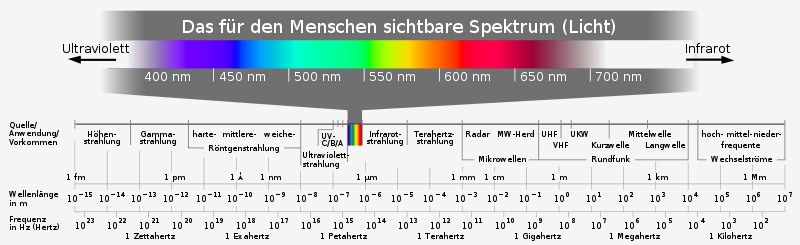
\includegraphics[width=\columnwidth]{pics/elektromagnetisches_Spektrum.png}
 \caption{Elektromagnetisches Spektrum mit dem für den Menschen sichtbaren Bereich des Spektrums.  \cite{elektromagnetisches_Spektrum}}
 \label{dsafigure:beispiel}
\end{dsafigure}

Das Sonnenlicht enthält alle Farben dieses Farbspektrums und erscheint deshalb weiß. Wenn die Lichtquelle ausgeschaltet ist, sehen wir schwarz, da kein Licht ausgestrahlt wird. Wird bei diesem additiven Farbsystem zum Beispiel das Licht von einer blauen und einer roten Lampe addiert, entsteht die Farbe Magenta (siehe Abbildung \ref{dsafigure:farbkreis}). Im Gegensatz dazu wird das Licht einer Lichtquelle (zum Beispiel der Sonne) von allen Gegenständen reflektiert. 
Bei diesem substraktivem Farbsystem ergibt sich die Farbe Schwarz aus der gemeinsamen Absorption von Wellenlängen aller Farben (siehe Abbildung \ref{dsafigure:farbkreis}).

Den Zusammenhang zwischen der Wellenlänge und der Energie lässt sich mit folgender Formel erklären:

\begin{equation}
E = \frac{h \cdot c}{\lambda} 
= h \cdot \nu
\end{equation}

$E$ beschreibt die Energie des Photons, $h$ das Plancksches Wirkungsquantum, $c$ die Lichtgeschwindigkeit, $\lambda$ die Wellenlänge, und $\nu$ die Frequenz.
Bei einer höheren Energie hat das Licht eine höhere Frequenz und dementsprechend ist die Wellenlänge kürzer. Umgekehrt bedeutet es auch, dass das Licht bei einer niedrigeren Energie eine niedrigere Frequenz und somit auch eine längere Wellenlänge hat.

\begin{dsafigure}
 \centering
 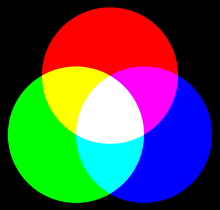
\includegraphics[width=0.45\columnwidth]{Additives_Farbsystem.png}
  \hfill
 
\includegraphics[width=0.45\columnwidth]{Substraktives_Farbsystem.png}
 \caption{Additives Farbsystem (links)\cite{Additives_Farbsystem} und Substraktives Farbsystem (rechts)\cite{Subtraktives_Farbsystem}}
 \label{dsafigure:farbkreis}
\end{dsafigure}


Der Zusammenhang zwischen Licht und Farbigkeit liegt an der Absorption und Reflexion von Licht. Dieses fällt durch die Pupille ins Auge und trifft dort auf die Netzhaut, die wiederum aus Stäbchen und Zapfen besteht. Die Stäbchen sind bei schwachen Lichteinfall aktiv und wir können damit nur schwarz-weiß sehen. Die Zapfen befinden sich im Zentrum der Netzhaut und sind besonders bei hohem Lichteinfall aktiv. Es gibt drei unterschiedliche Arten von Zapfen, die s-Zapfen, die als blaue Rezeptoren fungieren, die m-Zapfen, die als grüne Rezeptoren fungieren und die l-Zapfen, die als rote Rezeptoren fungieren. Jeder der Zapfen hat sein Maximum bei einer anderen Wellenlänge und zusammen decken sie somit den sichtbaren Bereich des elektromagnetischen Spektrums ab. 
Bei Anregung der Zapfen durch Licht, leiten sie einen Reiz an das Gehirn weiter. Durch die Kombination der verschiedenen angeregten Zapfen sehen wir Farbe.
Betrachten wir einen blauen Stift, der von der Sonne angeleuchtet wird, dann erscheint er uns blau. Was wir allerdings nicht sehen ist, dass die Elektronen im Stift vom Licht angeregt werden und vom Grundzustand in ein höheres Energieniveau angehoben werden (siehe Abbildung \ref{dsafigure:Grundzustand} ). Da dieser Zustand sehr instabil ist, fällt das Elektron wieder in seinen Grundzustand zurück. Dabei erfolgt die so genannten Relaxation über Schwingungen des Systems und es entsteht Wärme (siehe Abbildung \ref{dsafigure:Grundzustand}). Dass wir den Stift als blau wahrnehmen liegt daran, dass er die Komplementärfarbe zu Blau, also Gelb, absorbiert. Durch das fehlen der gelben Wellenlänge im reflektiertem Licht des Stiftes, interpretiert das Gehirn ihn als blau (siehe Abbildung \ref{dsafigure:farbkreis}, additives Farbsystem).
Wird blaues Licht durch einen Prozess emittiert, wird dieses ebenfalls als blau wahrgenommen.


\begin{dsafigure}
 \centering
 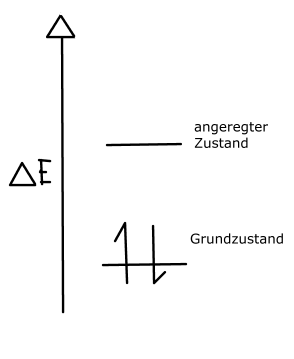
\includegraphics[width=0.45\columnwidth]{Grundzustand.png}
   \hfill
   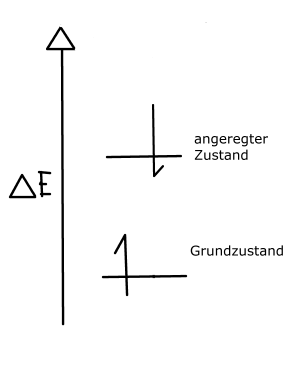
\includegraphics[width=0.45\columnwidth]{angeregter_Zustand.png}
 \caption{Elektronen im Grundzustand (links) und im angeregten Zustand (rechts)}
 \label{dsafigure:Grundzustand}
\end{dsafigure}


\section{Welle-Teilchen-Dualismus}

Autoren: Patricia Mühren, Kristina Heuser

Das Doppelspaltexperiment mit Photonen und Elektronen sowie der photoelektrische Effekt zeigen auf, dass Licht und Elektronen sowohl Wellen- als auch Teilchencharakter haben.

Zunächst kann das Doppelspaltexperiment mit Kugeln veranschaulicht und theoretisch betrachtet werden. Dabei werden Kugeln von einer Quelle ausgesendet und passieren zwei schmale, parallele Spalten. Auf einem Beobachtungsschirm in einiger Entfernung kann man daraufhin erkennen, dass die Verteilung beziehungsweise die Ankunftswahrscheinlichkeit für klassische Teilchen der Summe der beiden Einzelspaltverteilungen entspricht (vergleiche Abbildung \ref{dsafigure:beispiel1}). Im nächsten Schritt wird das Gedanken-Doppelspaltexperiment mit Wellen ausgeführt. Hier weist die Verteilung ein Interferenzmuster auf. Dies lässt sich dadurch erklären, dass die Maxima der Verteilungsfunktion genau an den Orten konstruktiver Überlagerung liegen (vergleiche Abbildung \ref{dsafigure:beispiel2}). 

\begin{dsafigure}
\centering
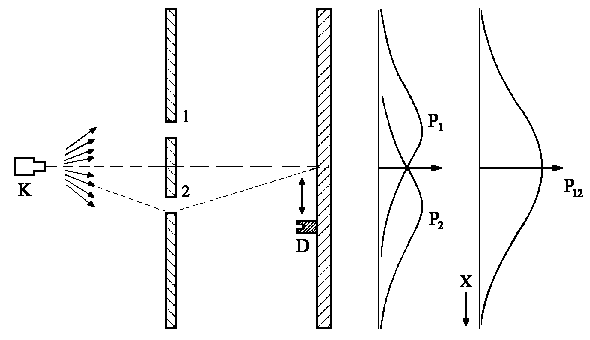
\includegraphics[scale=0.5]{Kugeln.png}
\caption{Das Doppelspaltexperiment mit Kugeln. \cite{Doppelspalt}}
\label{dsafigure:beispiel1}
\end{dsafigure}

\begin{dsafigure}
\centering
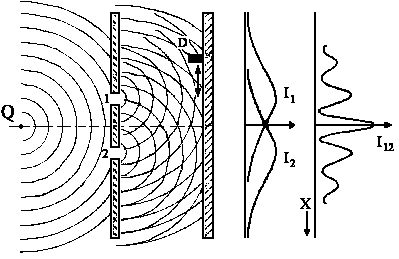
\includegraphics[scale=0.5]{Wellen.png}
\caption{Das Doppelspaltexperiment mit Wellen. \cite{Doppelspalt}}
\label{dsafigure:beispiel2}
\end{dsafigure}

Die Durchführung des Experimentes mit Elektronen zeigt, dass die Verteilungsfunktion der Elektronen nicht der Summe der beiden Einzelspaltverteilungen entspricht, wie sich Abbildung \ref{dsafigure:beispiel3} entnehmen lässt. Daher weisen Elektronen Welleneigenschaften auf. Ebenso zeigt Licht im Doppelspaltexperiment Interferenzen und, einhergehend damit, auch die Eigenschaften einer Welle. 

\begin{dsafigure}
\centering
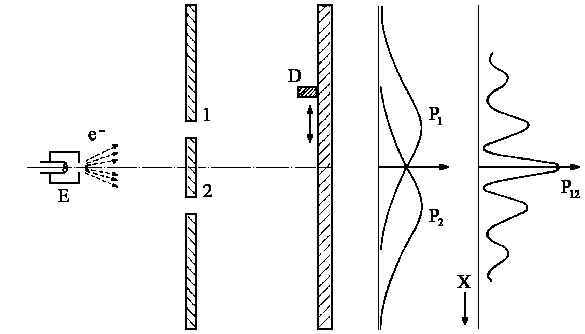
\includegraphics[scale=0.5]{Elektronen.png}
\caption{Das Doppelspaltexperiment mit Elektronen. \cite{Doppelspalt}}
\label{dsafigure:beispiel3}
\end{dsafigure}

Paradoxer Weise illustriert der photoelektrische Effekt, bei dem durch Auftreffen von Licht auf eine Metalloberfläche Elektronen emittiert werden, dass Licht ebenso Teilchencharakter aufweist, der der Wellennatur zuwider zu laufen scheint. Die Beobachtung gleichbleibender Energie der emittierten Elektronen bei zunehmender Intensität des Lichtes widerspricht der aus der klassischen Wellenbeschreibung abgeleiteten Folgerung, dass eine Zunahme der Intensität zu einem Anstieg der kinetischen Energie des herausgelösten Elektrons führen müsste. Dieser Umstand kann mit Teilchencharakter von Elektronen erklärt werden. Analog dazu wird derselbe Versuch mit Elektronen realisiert -- mit dem gleichen Ergebnis wie bei Licht.
Die Tatsache, dass Licht und Elektronen sowohl Wellen-, als auch Teilchencharakter besitzen, wird mit dem Welle-Teilchen-Dualismus addressiert. Sie ist aus einer rein klassischen Anschauung heraus nicht zu erklären und fordert eine neue Theorie \cite{Feynman_lectures70}.



\section{Die Schrödingergleichung}
\authors{Lena Trahe, Lynn Meeder}

Um die Struktur, Energie und Eigenschaften von Atomen und Molekülen zu beschreiben, bedient man sich der Quantenmechanik \cite{Reinhold}.

\subsection{Operatoren und Eigenwertprobleme}

Wendet man einen Operator $\hat{A}$ auf eine Funktion $f(x)$ an, so erhält man eine neue Funktion $g(x)$. Ein bekannter Operator ist zum Beispiel der Differentialoperator  $\frac{d}{dx}$.

Für einen solchen Operator lässt sich eine Eigenwertproblem formulieren, in dem $g(x)= af(x)$ und somit folgende Gleichung gilt:

\begin{equation}
\hat{A}f(x)=af(x)
 \label{OperatorEigenwert}
\end{equation}

Gesucht sind nun die Eigenfunktionen $f(x)$ und die Eigenwerte a, die Gleichung \ref{OperatorEigenwert} genügen.

\subsection{Zeitunabhängige Schrödingergleichung}

Die zeitunabhängige Schrödingergleichung ist das Eigenwertproblem des Hamilton-Operators $\hat{H}$:

\begin{equation}
\hat{H} \psi = E \psi
\end{equation}

Der Hamilton-Operator ist der Operator der Gesamtenergie $E$. Die Gesamtenergie ist die Summe aus kinetischer Energie $T$, die vom Impuls $\vec{p}$ abhängt, und potentieller Energie $V$, die vom Ort $\vec{x}$ abhängt. Analog ist der Hamilton-Operator die Summe aus den Operatoren für die kinetische und die potentielle Energie:

\begin{equation}
\hat{H}(\hat{\vec{p}}, \hat{\vec{x}}) = \hat{T} (\hat{\vec{p}}) + \hat{V} (\hat{\vec{x}})
\label{HamiltonOperatorTV}
\end{equation}

$\hat{\vec{p}}$ ist somit der Impulsoperator und $\hat{\vec{x}}$ der Ortsoperator. Die kinetische Energie $T$ wird in der klassischen Mechanik als $\frac{\vec{p}^2}{2m}$ beschrieben. Den Impulsoperator $\hat{\vec{p}}$ stellt man in der Quantenmechanik nun dar als 

\begin{equation}
\hat{\vec{p}} = -i\hbar \left( 
\begin{array}{c}
\frac{\partial}{\partial x} \\ \frac{\partial}{\partial y} \\ \frac{\partial}{\partial z}
\end{array} \right)
\end{equation}

Durch Einsetzen in den Ausdruck $\hat{T}=\frac{\hat{\vec{p}}^2}{2m}$ erhält man:

\begin{equation}
\hat{T}=-\frac{\hbar^2}{2m}  \left( \frac{\partial ^2}{\partial  x^2}+\frac{\partial ^2}{\partial  y^2}+\frac{\partial ^2}{\partial  z^2}\right)
\end{equation}

Die potentielle Energie hängt nur vom Ort $\vec{x}$ ab und ist deshalb in der Ortsdarstellung ein multiplikativer Operator: $\hat{V}(\hat{x})=\hat{V}(x)$. Die potentielle Energie eines Elektrons mit der Ladung $-e$ im Feld eines Protons mit der Ladung $+e$ beträgt $\hat{V}(x) = -\frac{1}{4 \pi \epsilon_0}\frac{e^2}{r}$. r bezeichnet die Entfernung des Elektrons zum Kern. Für das Wasserstoffatom lautet Gleichung \ref{HamiltonOperatorTV} also:

\begin{equation}
\left[ - \frac{\hbar^2}{2m}  \hat{\vec{\nabla}}^2 -\frac{1}{4 \pi \epsilon_0}\frac{e^2}{r} \right] \psi = E\psi
\end{equation}

Wobei der Operator $\hat{\vec{\nabla}}^2$ gegeben ist als:

\begin{equation}
\hat{\vec{\nabla}}^2 = \frac{\partial ^2}{\partial  x^2}+\frac{\partial ^2}{\partial  y^2}+\frac{\partial ^2}{\partial  z^2}
\end{equation}

Die diskreten Energieeigenwerte $E$ sind hier:

\begin{equation}
E_n=-\frac{m_e e^4}{2\hbar^2}\frac{1}{n^2} \:mit \: n\in \mathbb{N}
\end{equation}

\section{Koordinationsverbindungen II - Ligandenfeldtheorie}
\authors{Lynn Meeder, Patricia Mühren}

Die Kristallfeldtheorie beschreibt Koordinationsverbindungen, wobei die Liganden klassisch betrachtet werden und das Zentralatom/-ion quantenmechanisch beschrieben wird. Ein genaueres Modell ist die Ligandenfeldtheorie, in der sowohl das Zentralatom/-ion als auch die Liganden sowie ihre Wechselwirkungen quantenmechanisch betrachtet werden.

\subsection{Ligandenfeldtheorie und 18-Elektronen-Regel}

Analog zur Oktettregel lässt sich die 18-Elektronen-Regel für Nebengruppenelemente formulieren. Wenn das System 18 Valenzelektronen hat, so ist die Komplexbildung stabil \cite{Huheey}.

Die Liganden sorgen auch in diesem Modell, genau wie bei der Kristallfeldtheorie, für eine Aufspaltung der Energieniveaus der $d$-Orbitale des Zentralatoms/-ions. Dabei bilden die $d_{z^2}$- und $d_{x^2-y^2}$-Orbitale des Zentralatoms/-ions mit zwei symmetrieadaptierten Linearkombinationen (SALCs) der Liganden zwei bindende und zwei antibindende Orbitale. Die bindenden Orbitale liegen auf einem energetisch niedrigeren Niveau und werden als $e_g$-Orbitale bezeichnet. Auf einem höheren Energieniveau liegen die antibindenden $e^*_g$-Orbitale. Die energetisch niedriger liegenden $d_{xy}$-, $d_{xz}$- und $d_{yz}$-Orbitale  werden als $t_{2g}$-Orbitale bezeichnet und sind nicht bindend.

Das unbesetzte $s$-Orbital des Zentralatoms/-ions bildet mit einem der SALCs der Liganden das komplett symmetrische $a_{1g}$-Orbital und das entsprechende antibindende $a^*_{1g}$-Orbital. Die drei unbesetzten $p$-Orbitale des Zentralatoms/-ions bilden mit drei SALCs der Liganden die bindenden, dreifach entarteten $t_{1u}$-Orbitale und ebenfalls die entsprechenden antibindenden $t^*_{1u}$-Orbitale.

Die Aufspaltungsenergie $\Delta_0$ beschreibt die Energiedifferenz zwischen den $e^*_g$- und $t_{2g}$-Orbitalen (siehe Abbildung \ref{Level}).

\begin{dsafigure}
	\centering
	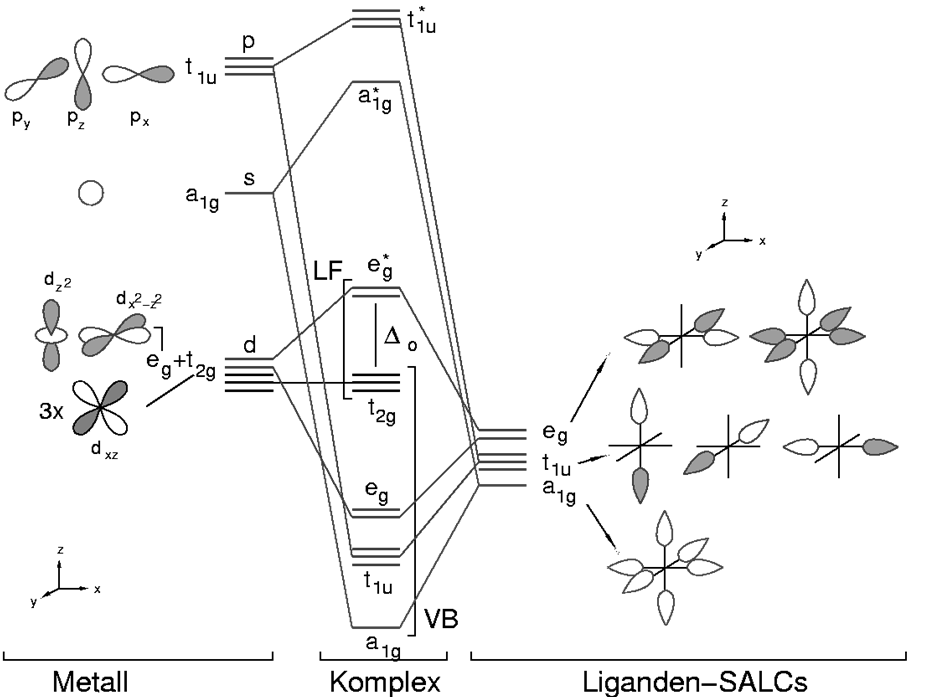
\includegraphics[width=\columnwidth]{EnergielevelKomplex.png}
	\caption{Die Molekülorbitale einer oktaedrischen Koordinationsverbindung \cite{Chemie_der_Metalle}}
	\label{Level}
\end{dsafigure}

Wie in Abbildung \ref{Level} sichtbar, gibt es sechs bindende und drei nicht bindende Orbitale. Die stärkste Bindung erhält man also, wenn diese neun Orbitale voll -- also mit 18 Elektronen -- besetzt sind. Damit lässt sich nun die 18-Elektronen-Regel begründen. 

Diese Regel gilt nun allerdings wie Abbildung \ref{Level}  nur für oktaedrische Komplexverbindungen. Bei anderen Koordinationsgeometrien unterscheidet sich das Molekülorbitalschema und dadurch kann eine andere Zahl an Valenzelektronen stabil sein.



\section{Hückeltheorie}

Autoren: David Bürg, Isabelle Schulte-Herbrüggen

Die Hückeltheorie wurde in den 1930er Jahren von Erick Hückel entwickelt. \cite{Reinhold} Sie erlaubt eine einfache Beschreibung von konjugierten Doppelbindungssystemen. Die Methode arbeitet mit vielen Näherungen. Daher ist sie zwar ungenau, aber einfach anzuwenden. Sie baut auf der Näherung von $\pi$-Molekülorbitalen und deren Energien über Linearkombinationen von p-Atomorbitalen auf. Die Linearkombinationen können mit:

\begin{align}
 \psi_{i} = \sum \limits_{k=1}^n c_{ik} \chi_k 
\end{align}

beschrieben werden. Der Koeffizient $c_{ik}$ gibt hierbei an, wie  stark die einzelnen Atomorbitale $\chi_k$ am Molekülorbital $\psi_i$ beteiligt sind. Die Koeffizienten $c_{ik}$ lassen sich über die Summen:

\begin{align}\label{eq:hueckel}
  \sum \limits_{k=1}^n (H_{jk}-\epsilon_i S_{jk}) c_{ik} = 0
\end{align}

bestimmen. $H_{jk}$ ist das Hamiltonmatrixelement, $S_{jk}$ das Überlappmatrixselement und $\epsilon_i$ ist die Energie des Molekülorbitals. Mit Gleichung (\ref{eq:hueckel}) kann nun die Hückelmatrix formuliert werden. Dabei wird angenommen, dass die Hamiltonmatrixelemente aller Kohlenstoffatome gleich sind, sowie dass die Wechselwirkungen aller nächsten Nachbarn gleich sind. Zusätzlich vereinfacht man die Beschreibung noch weiter, indem die Wechselwirkungen zwischen nicht-nächsten Nachbarn komplett vernachlässigt werden. Aufgrund dieser Vereinfachungen sind die Ergebnisse, die man durch Anwenden der Hückeltheorie erhält, grobe Näherungen.


Indem man fordert, dass die Determinante der Hückelmatrix verschwindet, erhält man einen Satz gekoppelter Gleichungen, deren Lösung die Koeffizienten $c_{ik}$ und die Orbitalenergien $\epsilon_i$ liefert. So kann nun die Energiedifferenz zwischen HOMO und LUMO mit:

\begin{align}
  \Delta E = \epsilon_{LUMO} - \epsilon_{HOMO}
\end{align}

berechnet werden. Diese Energiedifferenz erlaubt eine grobe Abschätzung der ersten Anregungsenergie des Moleküls.

Beschreibt man das 1,3-Butadien-Molekül mit der Hückelthoerie, erhält man die in Abbildung  \ref{fig:Hueckel_Butadiene} dargestellten Molekülorbitale.

\begin{dsafigure}
 \centering
 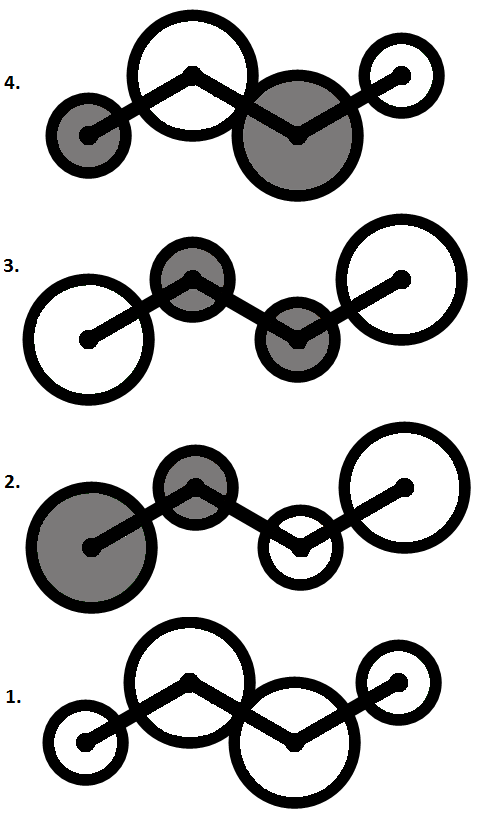
\includegraphics[width=8cm]{Hueckel_Butadiene.png}
 \caption{Aufsicht auf ein 1,3-Butadienmolekül. Schematische Darstellung der Hückelmolekülorbitale von 1,3-Butadien.}
 \label{fig:Hueckel_Butadiene}
\end{dsafigure}

Die Radien der Kreise entsprechen den Koeffizienten $c_{ik}$, während Weiß und Grau die Positivteile beziehungsweise Negativteile beschreiben. Das erste Orbital ist das energetisch günstigste Molekülorbital von Butadien, da es nur bindende Wechselwirkungen aufweist und keine Knotenebene besitzt; es ist ein bindendes Orbital. Das zweite Orbital hingegen weist zwei bindende Wechselwirkungen und eine Knotenebene auf. Es handelt sich auch hier um ein bindendes Orbital. Beim dritten un vierten Orbital handelt es sich um antibindende Orbitale. Das dritte Orbital zeigt zwei Knotenebenen und eine bindende Wechselwirkung und das vierte Orbital weist drei Knotenebenen und keine bindenden Wechselwirkungen auf. Sie haben also mehr Knotenebenen als bindende Wechselwirkungen. Die Energie vier Molekülorbitale nimmt in aufsteigender Reihenfolge zu.

\section{Phosphoreszenz}
\authors{Selin Güler, Joes Biburger}

Mit Phosphoreszenz wird die Emission von Licht bezeichnet, die auf einen Übergang von einem angeregten Triplett- in einen Singulett-Grundzustand zurückzuführen ist. 

Der Phosphoreszenzvorgang beginnt mit der Absorption eines Photons mit spezifischer Wellenlänge durch ein Molekül. Letzteres wird vom Grundzustand in einen angeregten Singulettzustand $(S_1)$, in dem alle Elektronen mit entgegengesetztem Spin gepaart sind, angeregt. Nun erfolgt der als Intersystem Crossing bezeichnete Übergang in einen angeregten Triplettzustand $(T_1)$. In diesem gibt es zwei ungepaarte Elektronen mit gleichem Spin. Der angeregte Triplettzustand $(T_1)$ ist energieärmer und somit stabiler als der angeregte Singulettzustand $(S_1)$. Aufgrund der Tatsache, dass die für den Übergang in den Grundzustand $(S_0)$ notwendige Spinumkehr spinverboten und somit unwahrscheinlich ist, können mehrere Stunden vergehen, bevor das Molekül in den Grundzustand zurückfällt. Bei einem solchen Übergang wird Energie in Form von Licht abgegeben. Das emittierte Licht ist immer langwelliger als das bei der Anregung aufgenommene. Das rührt daher, dass bei der Phosphoreszenz, ähnlich wie bei der Fluoreszenz, verschiedene Schwingungszustände innerhalb des Grund- $(S_0)$ sowie angeregten Triplettzustandes $(T_1)$ existieren. Das Molekül gibt beim Übergehen in den energieärmsten Schwingungszustand Energie strahlungsfrei an weitere Translations-, Rotations-, Schwingungsmoden ab, weshalb nur ein Teil der Energie des absorbierten Lichtes in Form von Licht wieder emittiert wird. 
\cite{Phosphoreszenz1}, \cite{Phosphoreszenz2}, \cite{Phosphoreszenz3}



\section*{Literaturverzeichnis}
\bibliographystyle{jcpsty_deutsch}
%\bibliographystyle{unsrtdin}
\bibliography{lit2}

\end{document}
